\documentclass[output=paper]{LSP/langsci} 
\ChapterDOI{10.5281/zenodo.1291940}
% \usepackage{rotating}
\title{Multilingual knowledge in aligned Wiktionary and OmegaWiki for translation applications}
 
\shorttitlerunninghead{Multilingual knowledge in aligned Wiktionary and OmegaWiki}

\author{Michael Matuschek\affiliation{Ubiquitous Knowledge Processing Lab (\textsc{ukp-tuda})}\and  Christian M. Meyer\affiliation{Ubiquitous Knowledge Processing Lab (\textsc{ukp-tuda})}\lastand  Iryna Gurevych\affiliation{Ubiquitous Knowledge Processing Lab (\textsc{ukp-tuda}, \textsc{ukp-dipf})}} 

\abstract{Multilingual lexical-semantic resources play an important role in translation applications. However, multilingual resources with sufficient quality and coverage are rare as the effort of manually constructing such a resource is substantial. In recent years, the emergence of Web 2.0 has opened new possibilities for constructing large-scale lexical-semantic resources. We identified Wiktionary and OmegaWiki as two important multilingual initiatives where a community of users (``crowd'') collaboratively edits and refines the lexical information. They seem especially appropriate in the multilingual domain as users from all languages and cultures can easily contribute. However, despite their advantages such as open access and coverage of multiple languages, these resources have hardly been systematically investigated and utilized until now. Therefore, the goals of our contribution are threefold: (1) We analyze how these resources emerged and characterize their content and structure; (2) We propose an alignment at the word sense level to exploit the complementary information contained in both resources for increased coverage; (3) We describe a mapping of the resources to a standardized, unified model (\textsc{uby-lmf}) thus creating a large freely available multilingual resource designed for easy integration into applications such as machine translation or computer-aided translation environments. %This resource is made available as integral part of \textsc{uby} at \url{http://www.ukp.tu-darmstadt.de/uby/}, while more information about the alignment is available at \url{http://www.ukp.tu-darmstadt.de/data/lexical-resources/wiktionary-omegawiki-alignment/}.
}
\maketitle
\begin{document}

\section{Introduction}
\largerpage
\label{sec:matuschek:intro}
In recent years, operating internationally has become increasingly important for governments, companies, researchers, and many other institutions and individuals. This raises a high demand for translation tools and resources. Statistical machine translation (\textsc{smt}) systems are pervasive nowadays and their use has become very popular (especially among layman translators), but they are usually hard to adapt to specific needs as parallel texts for training are not available for many domains, and even if training data is available the error rate is considerable. Thus, they are mainly useful during the gisting or drafting phase of translating a text, or as a supplementary tool to provide additional translations for a word or phrase. However, high quality translations as they are needed for many real-life situations still require human effort and editing \citep{Koehn09,Carl10}. \textsc{smt} systems are not sufficient for this purpose, since there is usually no hint of what the translations actually mean and why one alternative is preferable when only a bare probability score is 
provided. 

To produce translations of higher quality, additional tools and resources need to be considered. Translation Memory systems became very popular for this purpose in the 1990s \citep{Somers03}. They maintain a database of translations which are manually validated as correct and can be applied if the same or a similar translation is required. They can, to some extent, deal with unseen texts due to fuzzy matching, but while this approach yields a high precision, it cannot validate translations for entirely new content and is thus mostly useful in environments where the context does not change much over time. More recently, parallel corpora have been used to identify suitable translations in context; for example, through the \textit{Linguee}\footnote{\url{http://www.linguee.com}} service. While this might help in identifying the correct translation, pinpointing the exact meaning can be hard because no sense definitions or any other lexicographic information is provided. Moreover, the lack of 
sufficiently 
large parallel corpora is also an issue here.

We argue that to support translators directly and to improve \textsc{smt}, multilingual lexical resources such as bilingual dictionaries or multilingual wordnets (in addition to the tools mentioned) are required. Using the information in those multilingual resources (such as sense definitions), it becomes possible to manually or (semi-)automatically assess if a translation is appropriate in context and to perform corrections using a better suited translation found in the resource. As has been shown earlier, this is especially true for unusual language combinations and specific tasks such as cultural heritage annotation \citep{DBLP:conf/lrec/DeclerckML12, DBLP:conf/semweb/MoerthDLV11}.

 Consider, for example, the English noun \textit{bass}. In Google Translate,\footnote{\url{http://translate.google.com}} probably the most popular \textsc{smt} system to date, only the music-related word sense of \textit{bass} is considered for the example translation into German shown in \figref{google}. None of the translation alternatives addresses the less frequent animal-related word sense, which would be correct in this context. Moreover, there are no sense definitions or validated usage examples for the proposed translations.

In contrast, a multilingual lexical resource such as Wiktionary allows to easily distinguish between the two word senses of \textit{bass} and provides a vast amount of lexicographic information to help identify a good translation.  Although in this case of homonymy it would be comparatively easy to pick the correct sense, it poses a much greater problem for closely related senses sharing the same etymology. \figref{fig:basswkt} shows an excerpt of the animal-related word sense of \textit{bass} in Wiktionary that contains the suitable German translation \textit{Barsch} for the example discussed above. OmegaWiki encodes another possible translation \textit{Seebarsch} and provides additional lexicographic information. An excerpt is shown in \figref{fig:bassow}.
 
\begin{figure*} 
 \begin{center}
 \resizebox{\linewidth}{!}{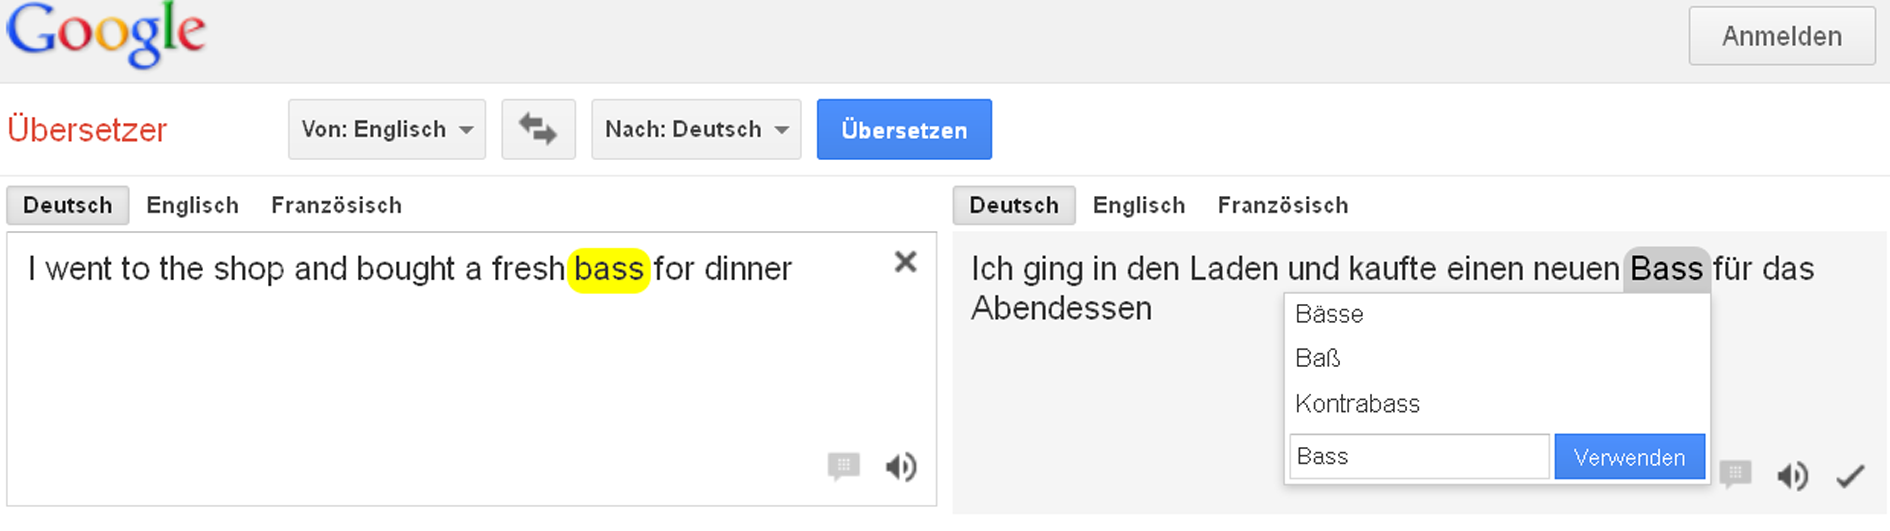
\includegraphics{figures/google3.png}}
 \caption{\label{google}
The translation alternatives for \textit{bass} in Google Translate, accessed on May 20th, 2011} 
 \end{center}
\end{figure*}



\begin{figure}
  
  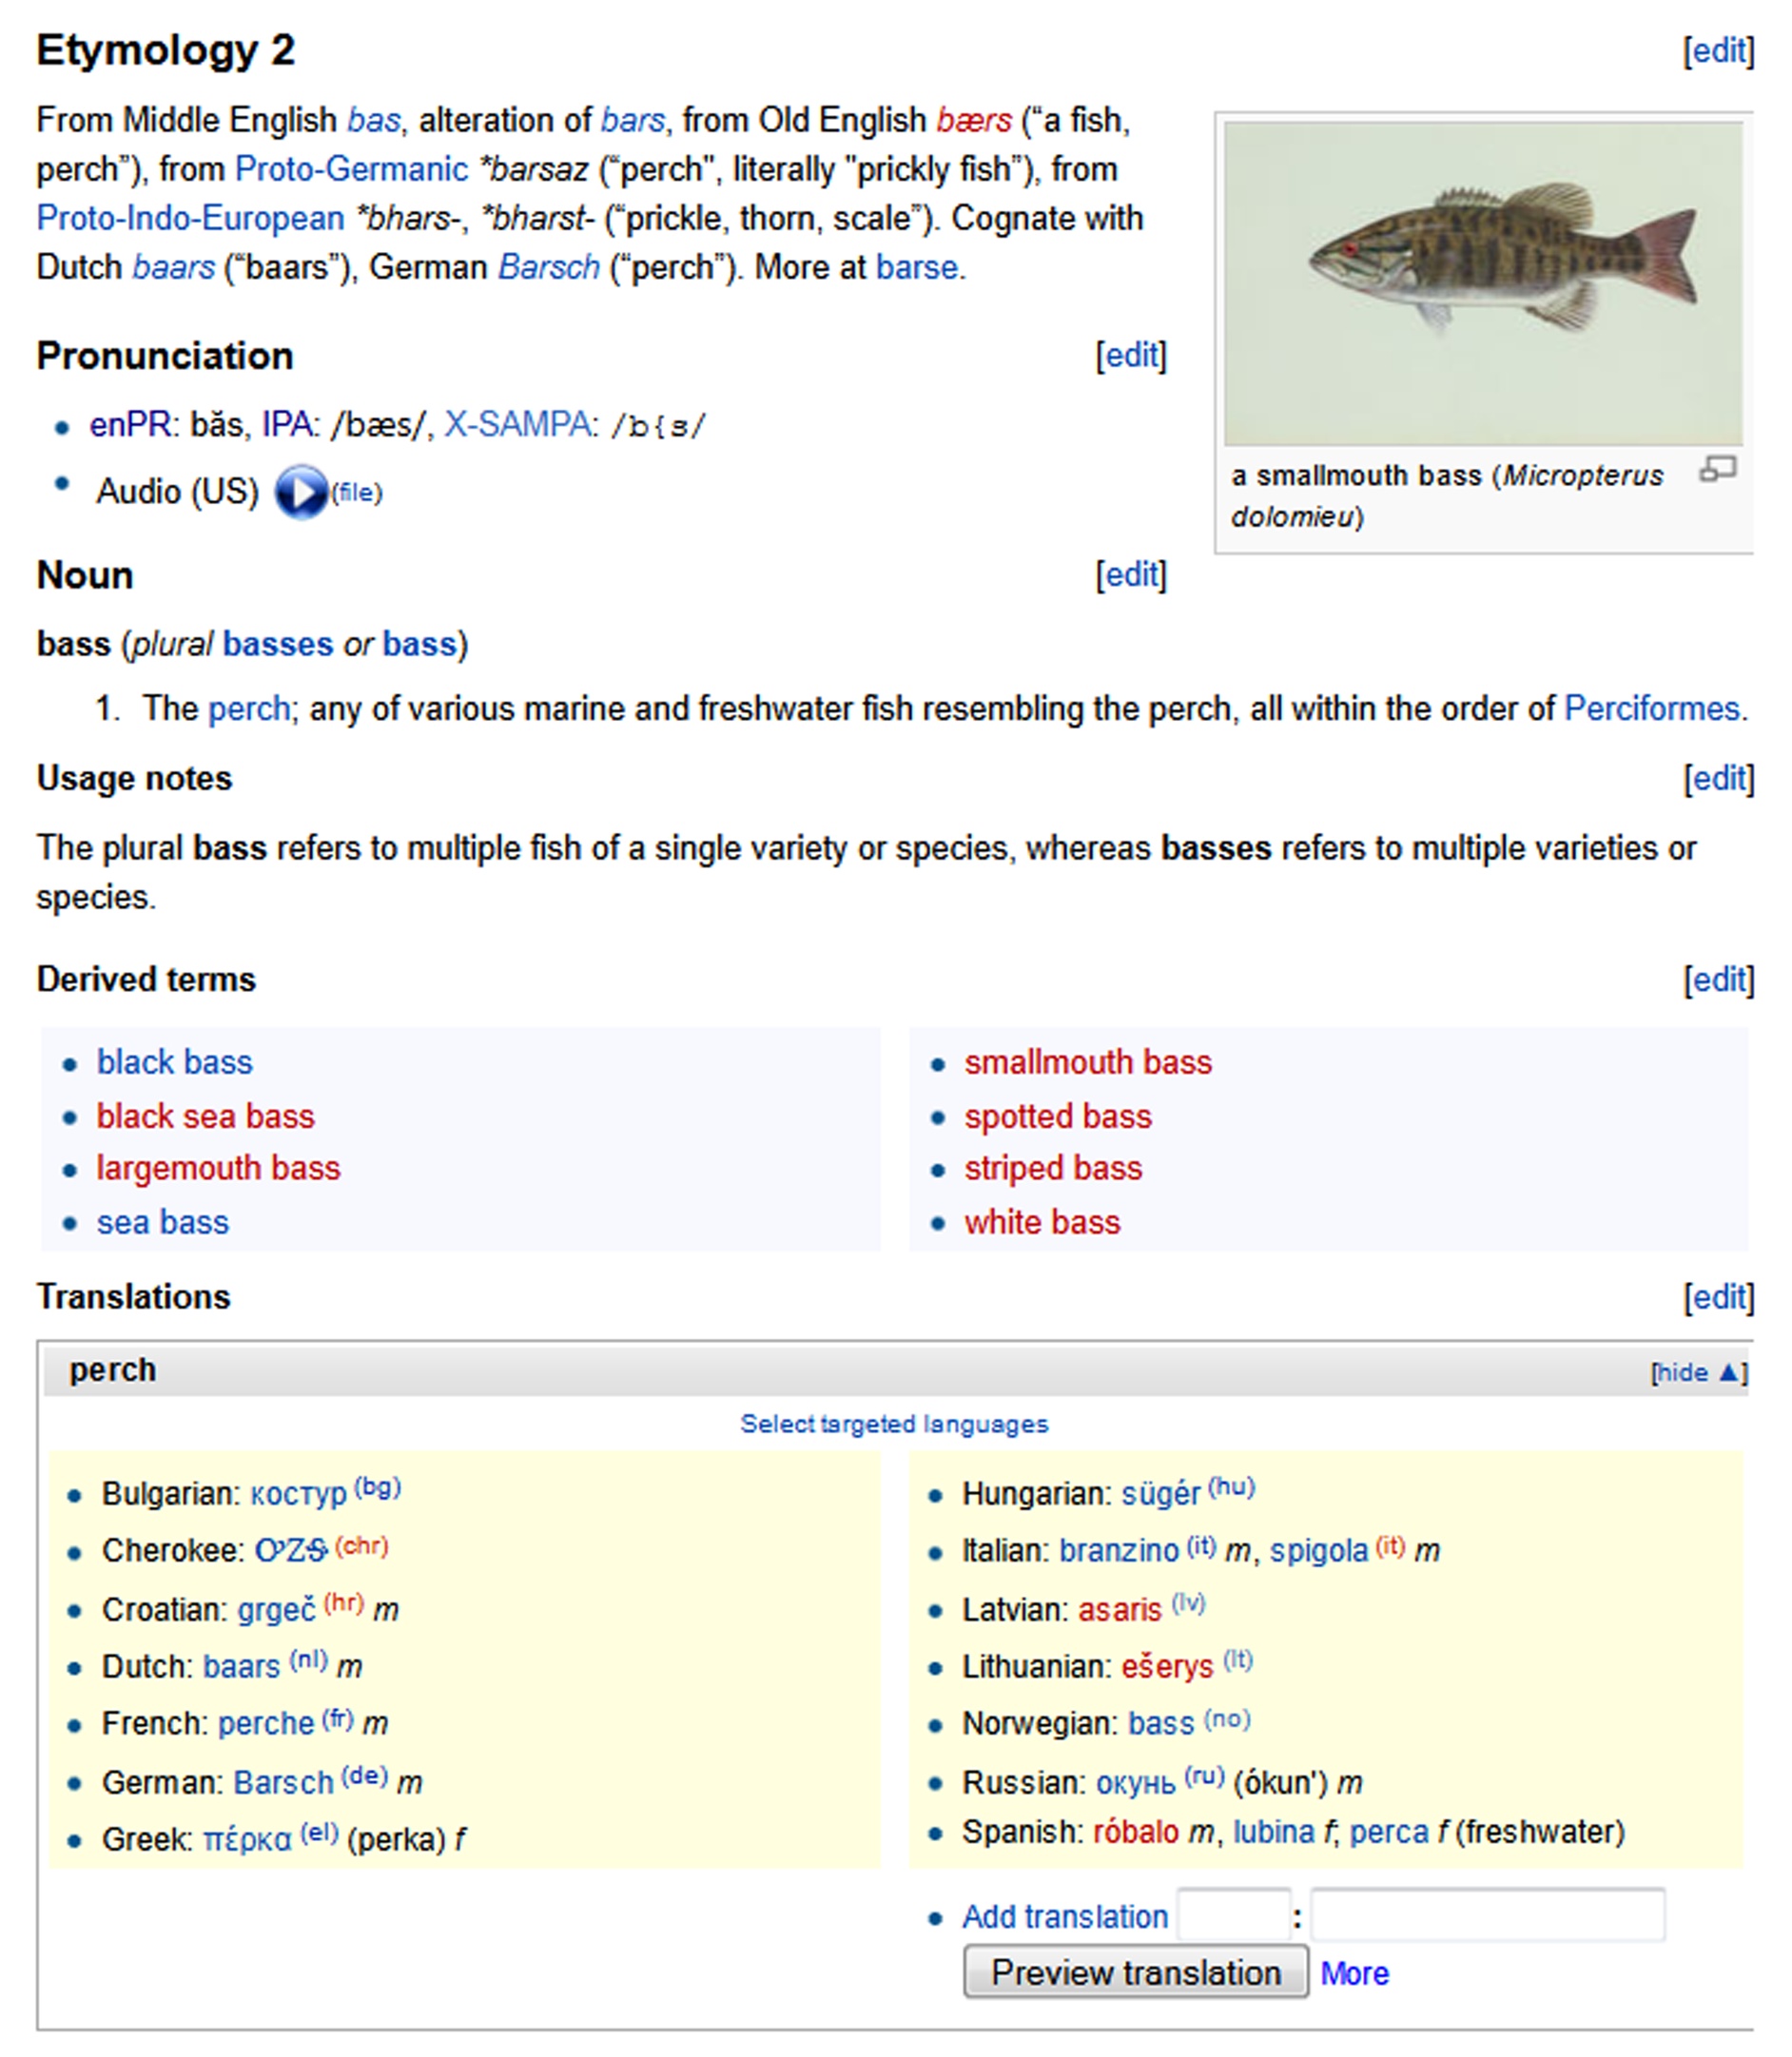
\includegraphics[width=\textwidth]{figures/basswkt.png}
  \caption{An excerpt of the Wiktionary entry on \textit{bass}. \url{http://en.wiktionary.org/wiki/bass}}
  \label{fig:basswkt}
\end{figure}

\begin{figure}
  
  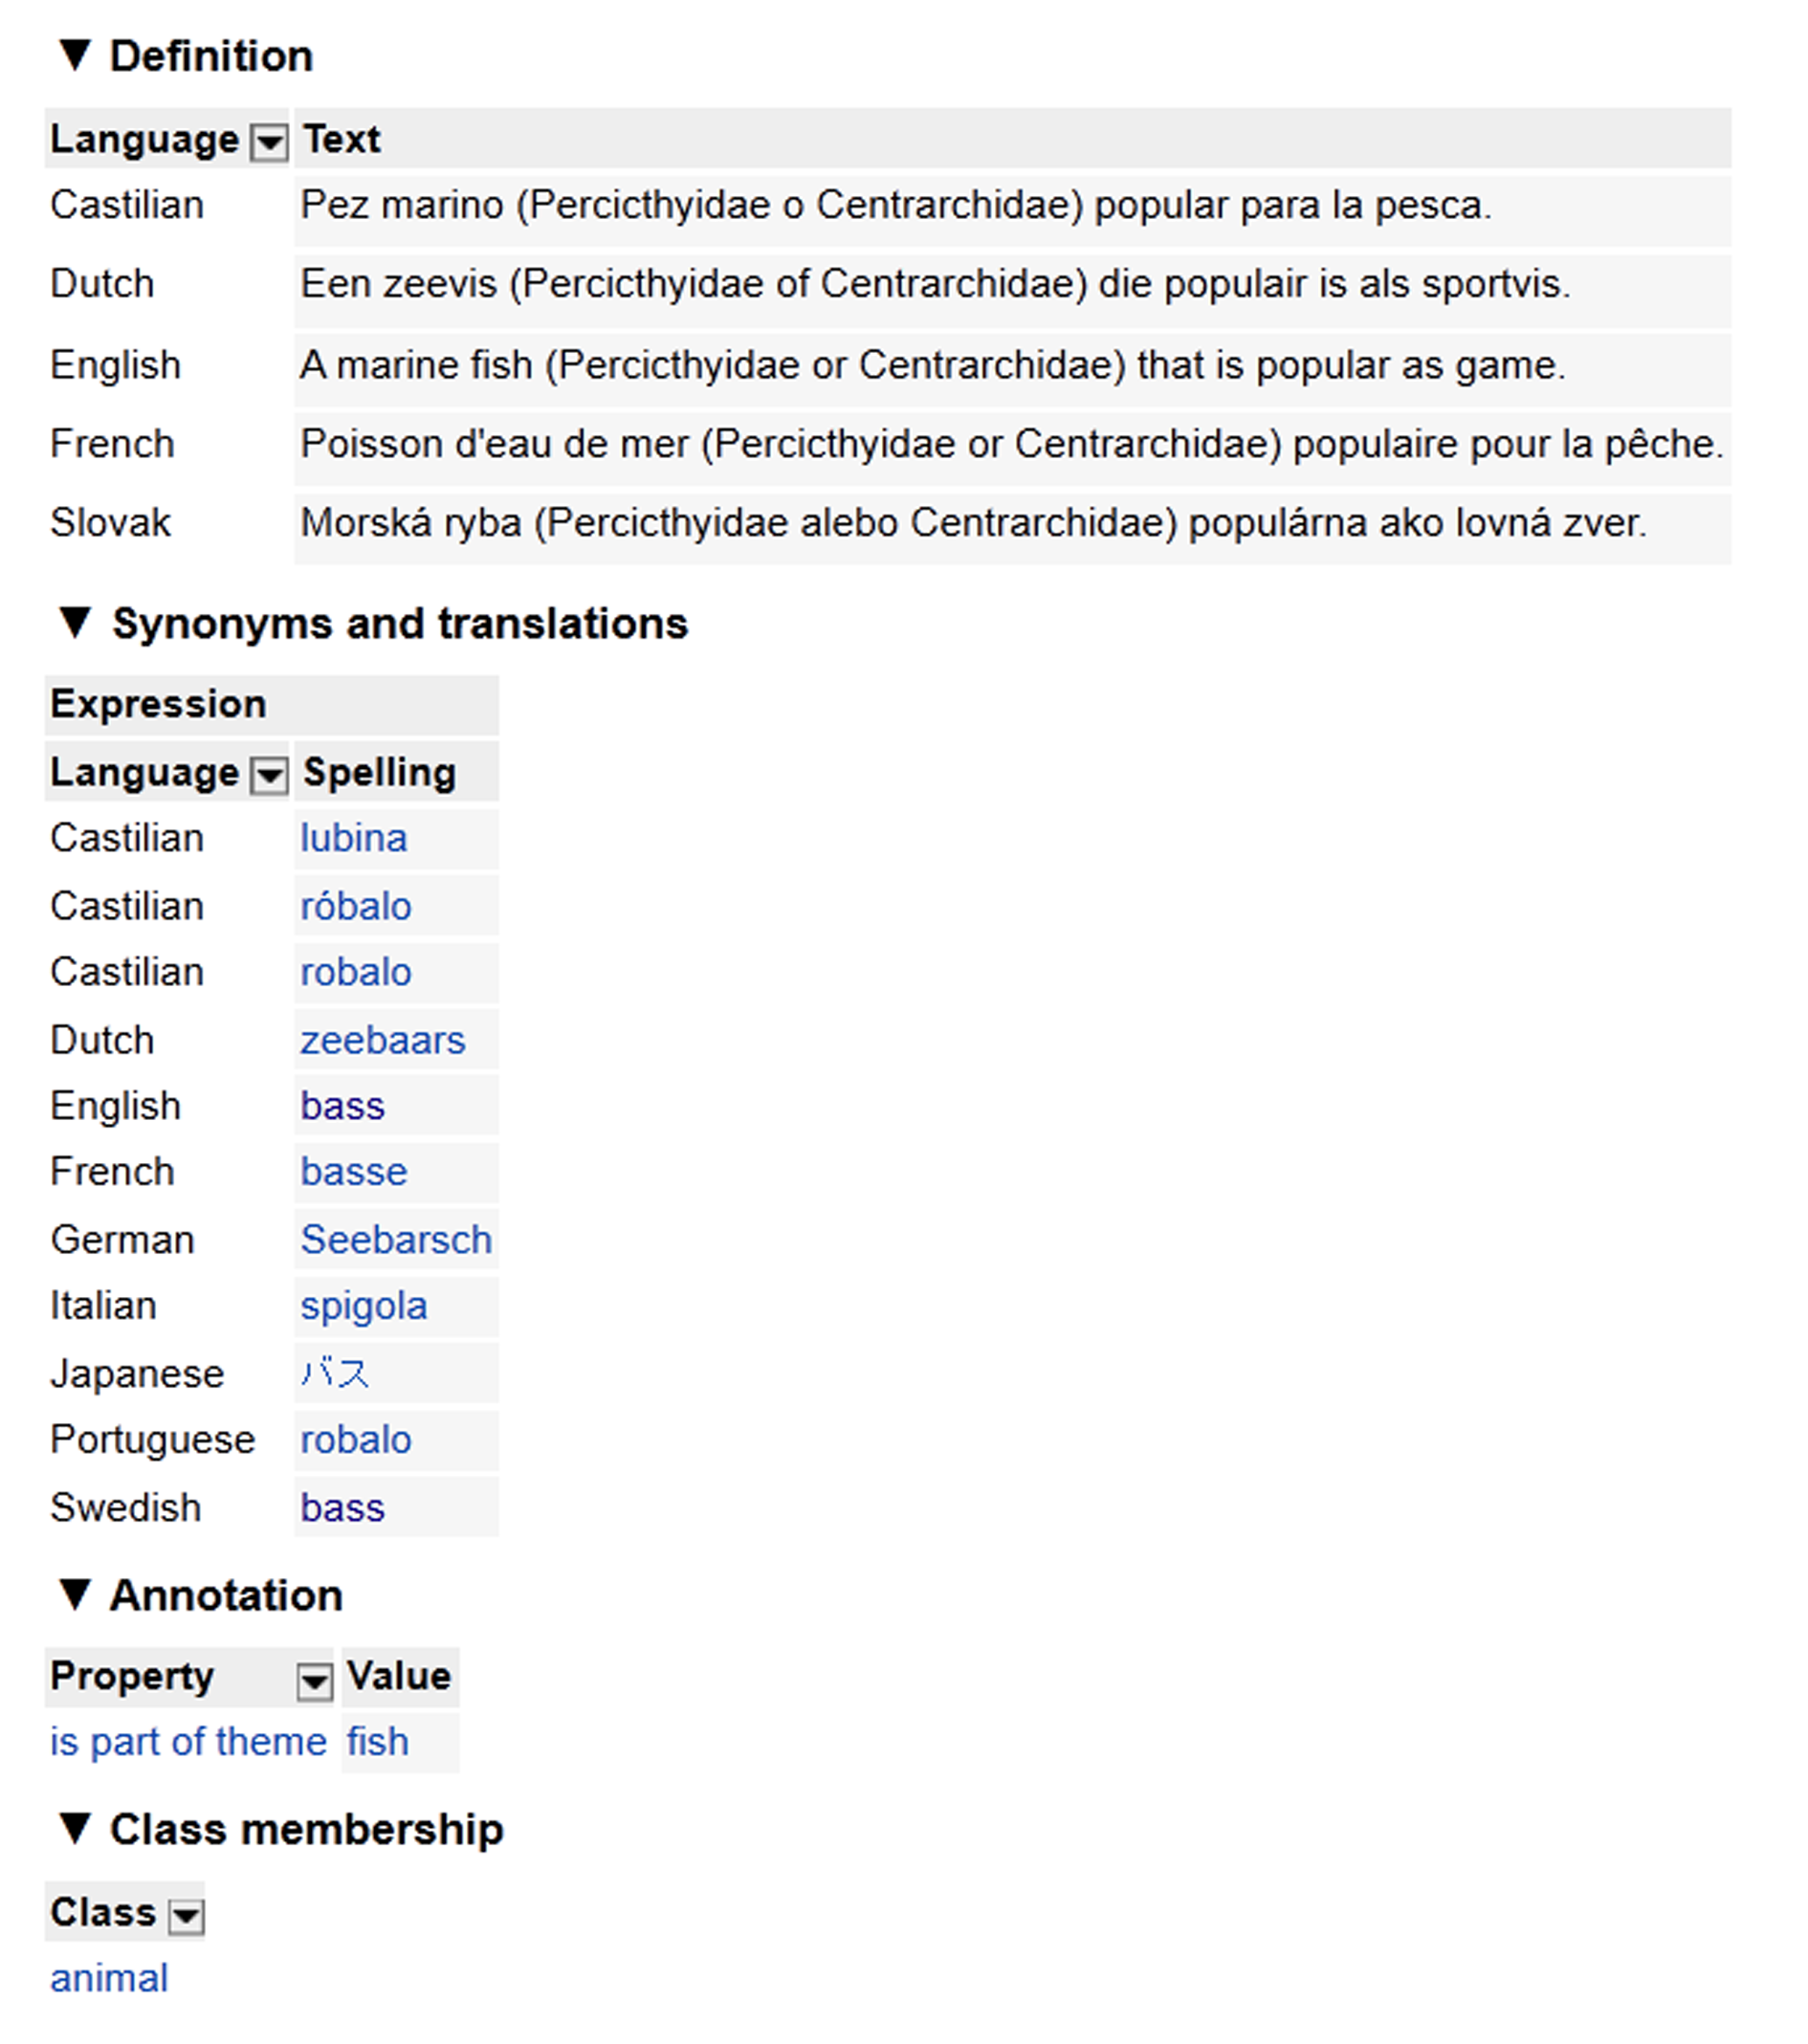
\includegraphics[width=\textwidth]{figures/bassow.png}
  \caption{An excerpt of OmegaWiki's Defined Meaning 5555 on \textit{bass}. \url{http://www.omegawiki.org/DefinedMeaning:bass_(5555)}}
  \label{fig:bassow}
\end{figure}


Among others, we identified the following three major requirements for such multilingual lexical resources to be useful for translation applications:

\begin{enumerate}
  \item The resources should have a high coverage of languages and allow for continually adding or revising information. This is important to cater for neologisms or domain-specific terminology, and especially for correcting improper or adding missing translations. Terminology-rich resources are especially important for human translators, as \textsc{smt} systems cannot cope well with domain-specific texts due to the lack of training data.
  \item There should be a large variety of lexicographic information types, such as sense definitions, example sentences, collocations, etc.\ that illustrate the use of a translation without being redundant. 
  \item Ideally, the resources should be seamlessly integrable into the translation environment via established standards and interfaces. 
\end{enumerate}

Most popular expert-built resources such as WordNet \citep{Fellbaum98} fail to fulfill some or all of these requirements. First of all, they need enormous building effort and are in turn rather inflexible with regard to corrections or addition of knowledge. This effort is also the reason why for many smaller languages such resources remain small or do not even exist.  Second, expert-built resources usually have a narrow scope of information types. WordNet focuses, for example, on synsets and their taxonomy, but mostly disregards syntactic information. Finally, many expert-built resources utilize proprietary or non-machine-readable formats, which make the integration into a translation environment difficult.

\noindent

In order to alleviate these problems, we study the collaboratively constructed resources Wiktionary\footnote{\url{http://www.wiktionary.org}} and OmegaWiki\footnote{\url{http://www.omegawiki.org}} and describe how multilingual lexical-semantic knowledge can be mined from and linked between these resources. This is meant as a first step to integrating them into \textsc{smt} systems, computer-aided translation
 systems, or other applications in the future. For the sake of illustrating our methodology, we focus on the English and German versions of these resources, but our results and insights can for the most part be directly applied to other languages. Among others, Wiktionary and OmegaWiki have the following advantageous properties:

\begin{description}\sloppy
\item[Easy contribution.] Wiktionary and OmegaWiki are based on a wiki system, which allows any Web user to contribute. This  crowd-based construction approach is very promising, since the large body of collaborators can quickly adapt to new language phenomena like neologisms while at the same time ensuring a remarkable quality -- a phenomenon known as the ``wisdom of crowds'' \citep{Surowiecki05}. 
\item[Good coverage of languages.] These resources are open to users from different cultures speaking any language, which is very beneficial to smaller languages. \citet{Meyer12a} found, for instance, that the collaborative construction approach of Wiktionary yields language versions covering the majority of language families and regions of the world, and that it covers a vast amount of domain-specific descriptions not found in wordnets.
\item[Free availability.] All the knowledge in these resources is available for free under permissive licenses. This is a major advantage of collaboratively constructed resources over efforts like EuroWordNet~\citep{Vossen1998}, where the aligned expert-built resources are subject to restrictive licenses. 
\end{description}

\noindent To our knowledge, the collaboratively constructed lexical resources OmegaWiki and Wiktionary have not yet been discussed in the context of translation applications. There exists a significant amount of previous work using Wikipedia in the context of cross-lingual information retrieval for query expansion or query translation \citep{EAMT2010,TUD-CS-2011-0067,Potthast:2008:WMR:1793274.1793338}, but it is primarily an encyclopedic resource, which limits the amount of lexical knowledge available for the application we address here. In previous work, \citet{TUD-CS-2009-0006} discussed combining Wiktionary and Wikipedia for cross-lingual information retrieval, but also in this case Wiktionary is merely used for query expansion and most of the lexicographic knowledge encoded in it remains disregarded. However, this knowledge is essential for translation applications in order to make well-grounded decisions. To fill this gap, we present the following four contributions in this article:

\begin{enumerate}
  \item We provide a comprehensive analysis of Wiktionary and OmegaWiki to characterize the information found therein, as well as their coverage and structure. 
  \item We automatically align Wiktionary and OmegaWiki at the level of word senses, that is we create a list of word senses in both resources which denote the same meaning so that we can benefit from the complementary lexicographic information types. For example, we aim at directly linking the animal-related word sense of \textit{bass} in Wiktionary to its corresponding sense in OmegaWiki -- but not to its music-related sense. As opposed to the mere linking at the lemma level, this is a non-trivial task because the resources differ greatly in the way they represent word senses (for example, different definition texts or varying granularity of senses).  Solving this issue allows us to effectively use the variety of lexicographic information found in both resources without being redundant.
  \item We standardize Wiktionary and OmegaWiki using the Lexical Markup Framework \citep{Francopoulo2009}. This is a necessary step for using those resources in natural language processing systems and for integrating them with other resources. 
  \item We create a sense-aligned unified resource containing the English and German versions of Wiktionary and OmegaWiki, serving as an example of how the standardization process can be operationalized. We publish this aligned resource as integral part of \textsc{uby} \citep{Gurevych12}, our unified lexical-semantic resource which is freely available at \url{http://www.ukp.tu-darmstadt.de/uby/}. The alignment between Wiktionary and OmegaWiki, along with accompanying information, is available at \url{http://www.ukp.tu-darmstadt.de/data/lexical-resources/wiktionary-omegawiki-alignment/} .
\end{enumerate}

\noindent
Since the data of Wiktionary and OmegaWiki is freely available with non-restric\-tive licenses, we are able to publish our sense alignment data and the standardized representation of the two resources. %Providing freely available multilingual resources is important for future research in translation applications.

Note that a task-based evaluation of our resulting resource is a crucial step to be taken. As this is still work in progress, we limit ourselves to presenting in detail the preparatory work that has been done with regard to analyzing, standardizing and combining Wiktionary and OmegaWiki. 

The remaining article is structured as follows: in the first part, we carry out our analysis of Wiktionary and OmegaWiki in \sectref{sec:matuschek:wiktionary} and \sectref{sec:matuschek:omegawiki} to familiarize the reader with these resources. After this, in \sectref{sec:matuschek:background}, we discuss previous work in the areas of multilingual resources, aligning them at the level of word senses, and using standardized models to represent them. Based on this, we introduce our work on aligning Wiktionary and OmegaWiki (\sectref{sec:matuschek:alignment}) and discuss how to represent them in a  standardized model (\sectref{sec:matuschek:lmf}), before we conclude our article in \sectref{sec:matuschek:conclusion}.


\section{Wiktionary}
\label{sec:matuschek:wiktionary}
\label{sec:matuschek:body}

\subsection{Overview}
Wiktionary is a publicly available multilingual dictionary. It is based on the wiki  
principle that users are free to add, edit, and delete (only with admin right) entries collaboratively."
entries collaboratively. Being a sister project of Wikipedia, gaining much attention, a rapid growth of dictionary articles ensued. Currently, Wiktionary is available in over 171 language editions providing more than 27.1 million articles (as of May 2018).   
The dictionary is organized in multiple \emph{article pages}, each of them covering the lexicographic information about a certain word. This knowledge includes the lexical class, pronunciations, inflected forms, etymology, sense definition, example sentences, translations, and many other information types commonly found in dictionaries. \citet{Meyer12a} give a more detailed introduction to the macro- and microstructure of Wiktionary.

Multilinguality is a key design feature of Wiktionary, which is implemented by two different notions:
\begin{enumerate}
  \item For each language, there is a separate Wiktionary \emph{language edition}, for instance, an English language edition available at \url{http://en.wiktionary.org} and a German language edition at \url{http://de.wiktionary.org}. The language of an edition determines the language of the user interface and of the encoded lexicographic information. 
  The German Wiktionary edition hence uses the German language for its browsing and search tools as well as its sense definitions, usage examples, etc.
  \item A language edition is not limited to words that are native to this language, but also allows the inclusion of \emph{foreign language entries}. There is, for instance, an entry about the German verb \textit{spazieren ge\-hen} in the English Wiktionary. The rationale behind this is to become able to use one's native language for describing foreign words; for example, describing the German verb as \textit{to take a stroll, to stroll, to take a paseo}. Defining foreign words in one's native language is important, as the actual native language definition \textit{sich in gem\"{u}tlichem Tempo zu Fu{\ss} fortbewegen, meist ohne Ziel} (English: \textit{to wander on foot at comfortable speed, often without specific destination}) is often beyond the language proficiency of a non-native speaker or language learner.\footnote{\raggedright\url{http://en.wiktionary.org/w/index.php?oldid=20466324} (12~May~2013), \url{http://de.wiktionary.org/w/index.php?oldid=2706581} (19~October~2012).}
\end{enumerate}
The different language editions are interlinked by \emph{translation links} and \emph{inter-wiki links}. The former are links between words with equivalent meanings in two languages. The German Wiktionary entry \textit{spazieren ge\-hen} has, for instance, an English translation \textit{(to) walk}. The latter is a link to the same word form in another language edition, for example, from the German Wiktionary entry \textit{spazieren ge\-hen} to the English Wiktionary entry \textit{spazieren ge\-hen}. Using the inter wiki links, we are able to extract sense definitions of a word in multiple languages. 

\tabref{tab:lang:trans} shows the number of translations found within the English and German Wiktionary (in comparison with OmegaWiki). The table also shows the number of languages for which at least one translation is encoded and the number of translations for the most frequently used languages. Most translations are found for languages spoken  worldwide, such as English, French, Spanish, etc. Languages with only a few number of speakers also have only a small number of translation links. Besides a country's main languages, sometimes also dialects and ancient languages (like Egyptian) are included. An important difference between the language editions are the translations into the Wiktionary's native language: there are no translations to English within the English Wiktionary,  while the German Wiktionary contains 69,135 translations into German. In the German edition, non-native entries are equipped with a translation into German. The entry for the English word \textit{boat} encodes, for 
instance,
 a translation \textit{Boot} into German. In the English edition, such translations are encoded as part of the definition texts. The number of languages seems to be extremely high, especially for the English Wiktionary. It should thus be noted that there are only a few translations for some of them.

\subsection{Wiktionary as machine-readable resource}

Wiktionary has been designed to be used by humans rather than machines. 
The entries are formatted for easy perception using appropriate font sizes and bold, italic, or colored text styles, while at the same time assuring that as much information as possible fits on a screen. 
For machines, data needs to be available in a structured manner in order to become able to obtain, for instance, a list of all translations or enumerating all English pronouns. 
This kind of structure is not explicitly encoded in Wiktionary, but needs to be inferred from the wiki markup of each article by means of an extraction software. The wiki markup is an annotation language consisting of a set of special characters and keywords that can be used to mark headlines, bold and italic text styles, tables, hyperlinks, etc.\ within the article. The four equality signs in ``====Translations===='' denote, for example, a small headline that usually precedes the list of a word's translations. Besides the mere formatting purpose, the wiki markup can be used by a software tool to identify the beginning of the translation section, which looks similar on each article page. The vast use of such markup structures allows us to extract each type of information in a structured way and use this kind of data in other contexts or process it automatically in natural language processing applications.

Although there are guidelines on how to properly structure a Wiktionary entry, it is permitted to choose from multiple variants or deviate from the standards if this can enhance the entry. This happens, for instance, for homonyms, which are distinguished by their differing etymology (as opposed to monosemous entries that do not require this distinction) and presents a major challenge for the automatic processing of Wiktionary data. Another hurdle is the openness of Wiktionary -- that is, the opportunity to perform arbitrary changes at any time. While a key to Wiktionary's success and rapid growth, this might cause major structural changes, which raises the need for constant revision of the extraction software.

There are multiple software tools available for extracting lexicographic knowledge from Wiktionary, such as \textsc{jwktl} \citep{Zesch2008}, Wikokit \citep{Krizhanovsky09}, or \textsc{wisigoth} \citep{Navarro2009}. We use \textsc{jwktl} for our work. This is the only one capable of extracting information from both the English and the German Wiktionary editions, which are the ones we focus on in this work.


\begin{table} 
  \begin{tabularx}{\textwidth}{Xrrrr}
    \lsptoprule
		      & \multicolumn{2}{c}{Wiktionary} &\multicolumn{2}{c}{OmegaWiki}\\\cmidrule(lr){2-3}\cmidrule(lr){4-5}
    Resource          &   En &    De &   En &   De \\
    \midrule
    Translations  & 190,055 & 449,517 &  335,173	& 304,590\\
    into Chinese &   5,067 &  10,194 &   4,377  & 4,248 \\
    into English &       0 &  63,006 & 0 & 56,471  \\
    into Finnish &  14,342 &   4,114 &   18,997 & 19,536   \\
    into French &   5,388 &  53,364 &  54,068  & 46,931\\
    into German &   8,342 &  69,135 &   56,471  & 0 \\
    into Italian &   3,243 &  26,759 & 27,499& 25,288  \\
    into Japanese &  11,905 &   7,883 & 10,879 &  11,088  \\
    into Spanish &   5,852 &  41,114 &  67,622 & 47,554  \\
    \midrule
    Languages                    &     597 &     234 &    279  &  265\\ 
    \lspbottomrule
  \end{tabularx}
  \caption{Number of translations for selected languages and the sum of languages for which translations are available in Wiktionary and OmegaWiki}
  \label{tab:lang:trans}
\end{table}

\begin{table}[t]

\begin{tabular}{lrr}
  \lsptoprule
   & Wiktionary & OmegaWiki \\
  \midrule
  Entries (Total) & 14,021,155 & 442,723\\
  Entries (English) & 2,457,506	& 55,182\\
  Entries (German) & 177,124 & 34,559\\
  Languages covered & >400	& 290\\
  Languages with >10.000 entries  & 54	& 12\\
 Information storing & Wiki Markup/\textsc{xml}	& Relational DB\\

  \lspbottomrule
\end{tabular}
\caption{Descriptive statistics about Wiktionary and OmegaWiki as of May 2011. Further statistics can be found on our website \url{http://www.ukp.tu-darmstadt.de/uby/}
}
\label{tab:data}
\end{table}

\section{OmegaWiki}
\label{sec:matuschek:omegawiki}
\subsection{Overview}

OmegaWiki is a lexical-semantic resource which is freely editable via its Web frontend. To alleviate Wiktionary's problem of inconsistent entries caused by the free editing, OmegaWiki is based on a fixed database structure which users have to comply to. It was initiated in 2006 and explicitly designed with the goal of offering structured and consistent access to lexical information, or as the creators put it: ``The idea of OmegaWiki was born out of frustration with Wiktionary.''\footnote{\url{http://www.omegawiki.org/Help:OmegaWiki}, accessed on June 20th, 2012.}

The central elements of OmegaWiki's organizational structure are language-in\-de\-pend\-ent concepts (so-called \textsc{defined meanings}) to which lexicalizations of the concepts are attached.  These can be considered as multilingual synsets. This way, no language editions exist for OmegaWiki as they do for Wiktionary. Rather, all multilingual information is encoded in a single resource. As an example, Defined Meaning no.~5616 carries the lexicalizations \textit{hand}, \textit{main}, \textit{mano}, etc. and also definitions in different languages which describe this concept, for example, \textit{That part of the fore limb below the forearm or wrist}. This method of encoding the multilingual information in a synset-like structure directly yields correct translations as these are merely lexicalizations of the same concept in different languages.

\tabref{tab:lang:trans} shows statistics about the translations between different languages that we derived from these multilingual synsets. As with Wiktionary, the number of languages into which translations are available should be taken with a grain of salt, as for many languages only very few translations exist. An important thing to note here is that the number of translations from English to German is the same as for the opposite direction. The reason is that translations only exist if a concept is lexicalized in both languages. The number of possible translations for a concept is then the product of the number of lexicalizations in either language, which is symmetric.

 A useful consequence of this concept-centered design for multilingual applications such as cross-lingual semantic relatedness is that semantic relations are unambiguously defined between concepts regardless of existing lexicalizations. Consider for example the Spanish term \textit{dedo}: it is marked as hypernym of \textit{finger} and \textit{toe}, although there exists no corresponding term in English. This might also be immediately helpful for translation tasks, since concepts for which no lexicalization in the target language exists can be described or replaced by closely related concepts. Exploiting this kind of information is not as easy in resources like EuroWordNet where concepts are linked across languages, but the respective taxonomies are different \citep{Jansen2004}. 

\subsection{OmegaWiki as machine-readable resource}
OmegaWiki is based on a fixed structure, manifested in an \textsc{sql} database. This fixed structure of OmegaWiki is proprietary in the sense that it does not conform to existing standards for encoding lexicographic information such as the Lexical Markup Framework. Plainly spoken, it was designed and over time extended in a ``grass-roots approach'' by the community to cater for the needs identified for such a multilingual resource.

While this approach to structuring the information is not easy to tackle in terms of interoperability, it still makes the use of this resource easier than for Wiktionary. The underlying database ensures straightforward structured extraction of the information and less error-prone results due to the consistency enforced by the definition of database tables and relations between them. This database structure is documented in the help pages. Most recently, we published a Java \textsc{api} for OmegaWiki (\textsc{jowkl}\footnote{\url{http://code.google.com/p/jowkl/}}) which enables the easy usage of OmegaWiki in applications without resorting to using plain \textsc{sql}. 

However, the fixed structure also has the major drawback of limited expressiveness. As an example, the coding of grammatical properties is only possible to a small extent; complex properties such as verb argument structures can not be encoded at all. Moreover, an extension of this structure is not easy, as this would, in many cases, require a reorganization of the database structure by administrators to which present and future entries would have to conform. While it could be argued that such information is outside of the scope of the resource and thus does not need to be reflected, the possibility given in Wiktionary to (in theory) encode any kind of lexicographic information using the more expressive wiki markup makes it more attractive for future extension. In OmegaWiki, the users are not allowed to extend the structure and thus are tied to what has been already defined. Consequently, OmegaWiki's lack of flexibility and extensibility, in combination with the fact that Wiktionary was already quite popular at its  
creation, has caused it to grow less rapidly (see \tabref{tab:data}). 

Despite the above-mentioned issues, we believe OmegaWiki is useful as a case study since it exemplifies how the process of collaboratively creating a large-scale lexical-semantic resource can be moderated by means of a structural ``skeleton'' in order to yield a machine-readable result for machine translation and related applications.

\section{Related work}
\label{sec:matuschek:background}

Previous work has been carried out in the areas of multilingual resources, sense alignment, and resource standardization. \tabref{tab:background:resources} summarizes the advantages and drawbacks of each type of resource which we discuss in greater detail below.

\begin{table}
  \resizebox{\textwidth}{!}{
  \begin{tabular}{lccccc}
    \lsptoprule
    Resource & Information & Lexicon  & Computational & Update & Quality \\
    type & types & size & usage & time &  \\
    \midrule
    Dictionaries     &  many & considerable & hard & long & very high \\
    Wordnets & limited & small & easy & long & very high \\
    \textsc{oie}-based & many & huge & easy & short & low \\
    Wikipedia & encyclopedic & large & medium & short & high \\
    Wiktionary & many & large & medium & short & high \\
    OmegaWiki & many & medium & easy & short & high \\
    \lspbottomrule
  \end{tabular}
  }
  \caption{Comparison of the advantages of different resource types (\textsc{oie} = Open Information Extraction)}
  \label{tab:background:resources}
\end{table}
 

\subsection{Multilingual resources}

Human translators traditionally utilize monolingual and bilingual dictionaries as a reference. Dictionaries provide many different kinds of lexicographic information, such as sense definitions, example sentences, collocations, idioms, etc. They are well-crafted for being used by humans, but pose a great challenge to using them computationally. Although machine-readable dictionaries allow processing their data automatically, computers are often overstrained to properly interpret the structure of an entry or resolve ambiguities that are intuitively clear to humans.

The Princeton WordNet \citep{Fellbaum98} is a lexical knowledge base designed for computational purposes. The great success of the project motivated the creation of a large number of multilingual wordnets, such as EuroWordNet \citep{Vossen1998}, BalkaNet \citep{Stamou02}, or MultiWordNet \citep{Pianta02}. While the nature of these resources seems to perfectly meet our requirements, none of these multilingual resources gained a significant size or provides as many different information types as dictionaries, such as etymology, pronunciation or derived terms.

A large problem of these expert-built resources (both dictionaries and wordnets) is their time-consuming and costly construction. The small number of experts, moreover, prevents timely updates featuring new or updated contents. Automatically induced resources based on the output of Open Information Extraction (\textsc{oie}) systems such as KnowItAll \citep{Banko07} can be huge and kept up to date at any time. However, those resources are not sense-disambiguated \textit{per se} and, due to the completely automatic creation process, limited in their quality.

Regarding collaboratively constructed resources, Wikipedia\footnote{\url{http://www.wikipedia.org}} has been found as a very promising resource for a multitude of natural language processing tasks \citep{Zesch2007,Medelyan09}. Possibly the most well-known works are \textsc{yago} \citep{Suchanek08}, DBpedia \citep{Bizer09}, and WikiNet \citep{Nastase10} that provide the Wikipedia data in different machine-readable formats. The large size of Wikipedia and the overall high quality of the articles make Wikipedia a promising resource for translation tasks -- for example, as a parallel corpus \citep{Adafre06} and for mining bilingual terminology \citep{Erdmann09}. However, the vast majority of information in Wikipedia is encyclopedic and almost entirely focusing on nouns. Translators also require lexicographic information types such as idioms, collocations, or usage examples as well as translations for word classes other than nouns -- most importantly verbs, adjectives, and adverbs. 

This is why we explore Wiktionary and OmegaWiki as two novel collaboratively constructed multilingual resources. 
Wiktionary and OmegaWiki combine the advantages of the other resources discussed above:

\begin{itemize}
  \item They contain multiple different lexicographic information types.
  \item They are of considerable size and available in a large number of languages.
  \item Their data can be processed automatically.
  \item They are continually revised by the community and thus allow for timely updates. 
  \item The information is provided by humans and therefore it is of higher quality than in resources that have been induced fully automatically. 
\end{itemize}


\noindent

\subsection{Word sense alignment}

There have been many works on aligning resources at the level of word senses,  as it is deemed more and more crucial for natural language processing to make use of complementary resources in an orchestrated manner; see for instance \citep{Shi05,Ponzetto10}.
Most of them propose aligning the Princeton WordNet to other resources in order to improve its coverage and introduce novel types of information. It has been aligned to Roget's thesaurus and the Longman Dictionary of Contemporary English \citep{Kwong98}, the \textsc{hector} corpus \citep{Litkowski99}, the Unified Medical Language System \citep{Burgun01}, \textsc{cyc} \citep{Reed02}, VerbNet and FrameNet \citep{Shi05}, as well as the Oxford Dictionary of English \citep{Navigli06}.

A large body of work addresses the alignment of WordNet and Wikipedia. Automatic methods have been explored for aligning WordNet synsets with Wikipe\-dia categories \citep{Toral09,Ponzetto09} and WordNet synsets with Wikipedia articles \citep{Ruiz05,Melo10,Navigli10,Niemann2011}.

In our own previous work, Wiktionary has been aligned to WordNet and FrameNet \citep{Meyer11a, TUD-CS-2013-0057, TUD-CS-2013-0082}, OmegaWiki has been aligned to WordNet \citep{Gurevych12, TUD-CS-2013-0057},  but they have not yet been aligned to each other. See \sectref{sec:matuschek:alignment} for details on our previously used alignment approach based on gloss similarity.

 We go beyond this previous work by applying this approach to an alignment between two collaboratively-constructed resources which are inherently more error-prone. This has not been addressed so far in the literature. It is a very challenging task, as word sense representations (such as glosses), granularities, etc. vary greatly between different resources and the similarity between them has to be assessed appropriately. This is also part of the reason why using WordNet as a pivot resource, although tempting, did not give satisfactory results in preliminary experiments. Another reason is the small number of word senses in the intersection of the three resources, which would render the resulting aligned resource very small.

\subsection{Standardized resources}

Previous work on the standardization of resources includes models for representing lexical information relative to ontologies \citep{Buitelaar09,McCrae11} and standardized single wordnets in English \citep{Soria09a}, German \citep{Henrich10a} and Italian \citep{Toral10} using the \textsc{kyoto} standard Lexical Markup Framework (\textsc{lmf}) \citep{Francopoulo2009}. Wiktionary has also been modeled in \textsc{lmf} \citep{Serasset12} and other formats \citep{DBLP:conf/lrec/DeclerckML12} recently. \textsc{lmf} defines a meta-model for lexical resources and has proven to be the most flexible and powerful approach for modeling such resources. 

\citet{Soria09a} define WordNet-\textsc{lmf}, an \textsc{lmf} model for representing wordnets used in the \textsc{kyoto} project, and \citet{Henrich10a} do this for the German wordnet. These models are similar, but they still present different implementations of the \textsc{lmf} meta-model, which hampers interoperability between the resources. With \textsc{uby-lmf} \citep{EckleKohler12}, we proposed a model for a broad variety of wordnets and dictionaries.

\citet{Serasset12} proposes a transformation of Wiktionary to \textsc{lmf}. However, this approach does not include all information encoded in Wiktionary -- translations, for instance, are modeled at the level of words rather than at the level of word senses. However, this is crucial for translators since words can have different translations with different meanings. The same holds for the approach proposed by \citet{McCrae12}, who focus on linking lexical information to ontologies and hence model only a small part of Wiktionary's lexicographic information in their \textsc{lmf} model. In contrast, we aim to cover all information contained in Wiktionary. \citet{DBLP:conf/lrec/DeclerckML12} represent Wiktionary data using the Text Encoding Initiative (\textsc{tei}) standard, an alternative to \textsc{lmf}. Although their model is able to represent translations and many other lexicographic information types found in Wiktionary, the model does, for example, not contain pronunciations. In addition to that, only a few major lexical resources 
have been encoded using the \textsc{tei} standard, which limits the interoperability with other resources. To our knowledge, OmegaWiki has not been modeled in a standardized format by anyone else so far.

In \sectref{sec:matuschek:lmf}, we will discuss the \textsc{uby-lmf} model \citep{EckleKohler12} in detail as this is the model we base our unified model of Wiktionary and OmegaWiki on.

\section{Word sense alignment of Wiktionary and OmegaWiki}
\label{sec:matuschek:alignment}
As we have seen in \sectref{sec:matuschek:wiktionary} and \sectref{sec:matuschek:omegawiki}, the structures of Wiktionary (loosely defined and changeable by users) and OmegaWiki (fixed and well-defined) are quite different, and to some extent this is also true for their content. While Wiktionary offers a greater coverage and a richer variety of encoded information, OmegaWiki provides the advantage of unambiguous translations and relations which are potentially useful in translation applications. Thus, a crucial  next step for exploiting both resources is combining them, or, more specifically, aligning them at the word sense level. This offers various advantages:
\begin{itemize}
\item Better coverage as the information from both resources can be considered.
\item Exploitation of complementary information such as additional example sentences for a sense which help choosing the correct translation or additional translations contained in the additional resource.
\item Better structuring of translation results, for example, by clustering the translations into the same language for aligned senses instead of simply considering all of them in parallel.
\item Identical translations  in both resources yield combined evidence and thus higher translation confidence; the redundancy in the displayed results can be avoided by collapsing these translations.
\end{itemize}

\begin{figure*} [!ht]
 \begin{center}
 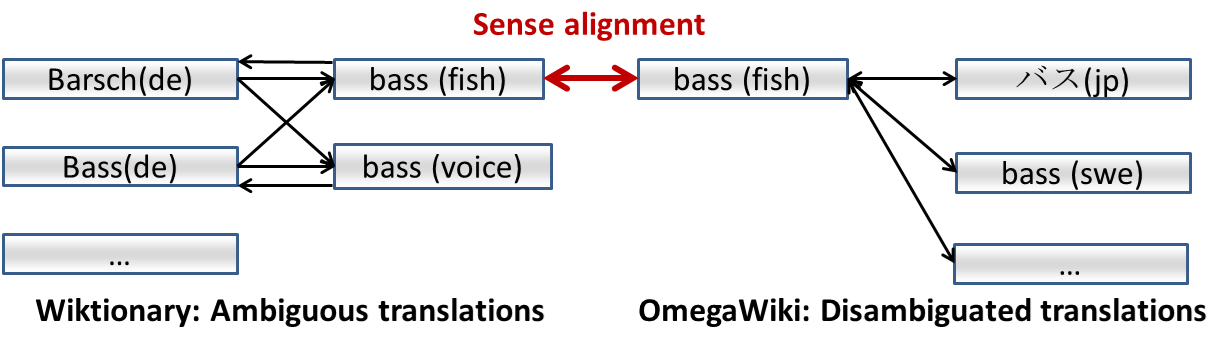
\includegraphics[width=\textwidth]{figures/OWWKT2}
 \caption{\label{alignment}Illustration of the sense alignment between Wiktionary and OmegaWiki. As the translations in OmegaWiki are unambiguous, they directly apply to the aligned Wiktionary sense. Although this is not the case for the translations in Wiktionary, they still offer additional translation options. The ambiguity in Wiktionary is exemplified by the arrows pointing from German ``Barsch'' and ``Bass'' to both English senses of ``bass'' -- there is no explicit link to the correct sense, only to the lexeme.}
 \end{center}
\end{figure*}
 

In this paper we align the English Wiktionary with OmegaWiki. As English is the language with the most entries in both resources, such an alignment yields the largest resulting resource and thus the greatest benefit. Moreover, there are no errors introduced into the alignment process by using machine translation, which would be a prerequisite for automatic cross-lingual alignment. 
As Omega\-Wiki is a multilingual resource by design, if Wiktionary (or any other resource) is aligned to OmegaWiki, we obtain an alignment to multilingual synsets -- this means that the (disambiguated) translations encoded here apply to the aligned Wiktionary senses. This entails that the correct translation is immediately known once the word sense in the source document can be correctly identified, either by the user or by automatic word sense disambiguation. A similar argument also holds for Wiktionary -- all aligned senses from OmegaWiki benefit from the additional translations available in Wiktionary. The only disadvantage in this case is that these are not disambiguated. This alignment is illustrated in \figref{alignment}.

In the remaining section, we will present the alignment algorithm, evaluate the results and present examples where the combination of resources is beneficial.

\subsection{The alignment procedure}
Creating sense alignments between multilingual lexical resources automatically is a challenging task because of word ambiguities and different granularities of senses \citep{Navigli06}. For aligning Wiktionary and OmegaWiki, we used the flexible alignment framework described in \citet{Niemann2011}. The framework supports this task for a large number of resources across languages and allows alignments between different representations of senses as found in different resources, for example WordNet synsets, FrameNet frames or even Wikipedia articles. The only requirement is that the individual sense representations are distinguishable by a unique identifier in each resource. 

The basic idea of the algorithm is, in a nutshell:
\begin{enumerate}
 \item For each sense in one resource, all possible candidates in the other resource are retrieved, and a similarity score between the glosses is calculated. For instance, for the \emph{programming} sense of \textit{Java} in Wiktionary, the \emph{programming}, \emph{island} and \emph{coffee} senses in OmegaWiki are considered.
\item For a subset of these (the gold standard), the alignment decision is manually annotated, and based on this, we can learn an optimal (in terms of F-measure) similarity threshold, that is the minimum similarity that is necessary for an alignment to be considered correct. 
\item Using this threshold learned from the gold standard, the alignment decision is made for all candidates to produce a complete alignment of the resources.
\end{enumerate}

In this case, we first extract OmegaWiki Defined Meaning candidates for each entry in the English Wiktionary. This is solely based on the combination of lemma and part-of-speech, that is, in the first step all senses for a word are considered potential candidates. Second, we create a gold standard by manually annotating a subset of candidate pairs as ``valid'' or ``non-valid''. Note that due to different granularities in these resources, it is well possible that $m:n$ alignments occur when, for example, one Wiktionary sense corresponds to several OmegaWiki senses. Then, we extract the sense descriptions to compute the similarity of word senses with two similarity measures: 

 (i) The \textsc{cosine similarity} (\textsc{cos}) calculates the cosine of the angle between a vector representation of the two senses $s_1$ and $s_2$:
 $$\operatorname{COS}(s_1, s_2) = \frac{\operatorname{BoW}(s_1) \cdot \operatorname{BoW}(s_2)}{||\operatorname{BoW}(s_1)|| \: ||\operatorname{BoW}(s_2)||}$$

 To represent a sense as a vector, we use a bag-of-words approach -- that is, a vector $\operatorname{BoW}(s)$ containing the term frequencies of all words in the description of $s$. 
Note that there are different options for choosing the description of sense $s$. 
For Wiktionary, we selected the gloss, usage examples, and related words of the word sense. For OmegaWiki, we chose the gloss, usage examples, and synonyms in the same language.
 
 (ii) The \textsc{personalized PageRank based measure  (ppr)} \citep{Agirre2009} estimates the semantic relatedness between two word senses $s_1$ and $s_2$ by representing them in a semantic graph and comparing the semantic vectors $\mathbf{Pr}_{s_1}$ and $\mathbf{Pr}_{s_2}$ by computing
 
 $$\operatorname{PPR}(s_1, s_2) = 1 - \sum_{\raisebox{-1.3ex}{\scriptsize $i$}} \frac{(\mathbf{Pr}_{s_1,i} - \mathbf{Pr}_{s_2,i})^2}{\mathbf{Pr}_{s_1,i} + \mathbf{Pr}_{s_2,i}}$$
 
 which is a $\chi^2$ variant introduced by \citet{Niemann2011}.
 The main idea of choosing $\mathbf{Pr}$ is to use the personalized PageRank algorithm for identifying those nodes in the graph that are central for describing a sense's meaning. 
 These nodes should have a high centrality (that is, a high PageRank score), which is calculated as 

 $$\mathbf{Pr} = c \, M \, \mathbf{Pr} + (1 - c) \, \mathbf{v}$$

 with the damping factor $c$ controlling the random walk, the transition matrix $M$ of the underlying semantic graph, and the probabilistic vector $\mathbf{v}$, whose $i\text{th}$ component $\mathbf{v}_i$ denotes the probability of randomly jumping to node $i$ in the next iteration step.\footnote{We use the publicly available \textsc{ukb} software  \citep{Agirre2009} for calculating the PageRank scores and utilize the WordNet 3.0 graph augmented with the Princeton Annotated Gloss Corpus as $M$. The damping factor $c$ is set to $0.85$.} Unlike in the traditional PageRank algorithm, the components of the jump vector $\mathbf{v}$ are not uniformly distributed, but personalized to the sense $s$ by choosing $\mathbf{v}_i = \frac{1}{m}$ if at least one lexicalization of node $i$ occurs in the definition of sense $s$, and $\mathbf{v}_i = 0$ otherwise. The normalization factor $m$ is set to the total number of nodes that share a word with the sense descriptions, which is required for obtaining a probabilistic vector.

\subsection{Aligning Wiktionary and OmegaWiki}
The candidate extraction process yielded 98,272 unique candidate sense pairs overall, covering 56,111 Wiktionary senses and 20,674 OmegaWiki Defined Meanings (that is, synsets containing one or more senses). 
When we consider the over 400,000 word senses in Wiktionary and the over 50,000 senses in OmegaWiki, this confirms that there is a considerable lexical overlap between the two resources, as well as a large number of entries which are  only  available in either one of the resources. This suggests that a combination of the resources indeed leads to a significantly increased coverage.
 
For creating the gold standard, we randomly selected 500 Wiktionary senses, yielding 586 candidate pairs. These were manually annotated by a computational linguistics expert as representing the same meaning (190 cases) or not (396 cases). This gold standard was used for training the threshold-based machine learning classifier and the subsequent evaluation with 10-fold cross-validation. Note that the threshold was optimized for F-measure; optimizing for precision would have led to higher thresholds and thus fewer alignments. \tabref{tab::validation} summarizes the results for the different similarity measures and their combinations in terms of precision $P$, recall $R$, and $F_1$ measure (the harmonic mean of precision and recall). The results of a random baseline are given for comparison. As there is no explicit sense frequency information encoded in either resource, the application of a most frequent sense baseline is not possible. We also considered using the existing alignments to WordNet to 
directly infer an alignment between Wiktionary and OmegaWiki using WordNet as pivot, but the different sense granularities in combination with small lexical intersection of all three resources rendered this approach very ineffective.  

\begin{table}
  
\begin{small}
  \begin{tabular}{lccc}
    \lsptoprule
    Similarity measure & $P$ & $R$ & $F_1$ \\
    \midrule
  Random & $0.542$ & $0.473$ & $0.489$ \\
     \textsc{cos} & $0.774$ & $0.771$ & $0.773$ \\
     \textsc{ppr}  & $0.745$ & $0.582$ & $0.582$ \\
     \textsc{ppr + cos}  & \textbf{0.782} &\textbf{0.783} & \textbf{0.783} \\
    \lsptoprule
  \end{tabular}
  \caption{Alignment results}
  \label{tab::validation}
\end{small}
\end{table}

We observe that the more elaborate similarity measure \textsc{ppr} yields worse results than cosine similarity (\textsc{cos}), while the best result is achieved by a combination of both. However, this difference between \textsc{cos} and the combination of \textsc{cos} and \textsc{ppr} is not statistically relevant at the $1\%$ level (McNemar test). These results differ from those reported in our earlier work which might be due to the fact that, by our observation, some sense definitions in OmegaWiki have been copied or adapted from Wiktionary, so that Cosine similarity alone already gives a very strong hint towards the correct sense. All measures outperform the random baseline by a huge margin.

 The F-measure of 0.783 in the best configuration is above the results we reported in \citet{Meyer11a} (0.66) and \citet{Niemann2011} (0.78) for alignments between Wiktionary and WordNet and Wikipedia and WordNet, respectively. 
The application of the trained classifier to all candidate pairs leads to a final alignment of 25,742 senses between Wiktionary and OmegaWiki.

\subsection{Error analysis}

We carried out an error analysis to identify the main errors made by our alignment algorithm. Of the 586 sense pairs in the gold standard, the classifier yielded 71 false positives (that is, incorrectly aligned senses) and 69 false negatives (that is, senses which should have been aligned but were not).

For the false positives, the main error we identified is that different senses were aligned because of very similar sense descriptions expressing only a slight difference which is hard to grasp for our approach. An example for this are two senses of \textit{(to) carry}: (1) \textit{To lift (something) and take it to another place; to transport (something) by lifting} (2)  \textit{To transport with the flow}. 

For the false negatives, we could basically identify two categories of errors:

\begin{enumerate}
\item Different sense descriptions for the same concept. These are not easy to tackle as a certain degree of understanding and world knowledge would be required. An example for this are two senses of the adjective \textit{aware} which should have been aligned, but were not because of insufficient overlap: (1) \textit{Conscious or having knowledge of something} (2) \textit{noticing something; aware of something}.

\item Short definitions making references to other, closely related or derived words. An example are these two definitions of \textit{alluvial}: (1) \textit{Pertaining to the soil deposited by a stream} (2) \textit{Of or relating to alluvium}. Without resolving the definition of the derived word a disambiguation is nearly impossible. This is, however, another word sense disambiguation problem which cannot be easily solved. 
\end{enumerate}


\subsection{Discussion of alignment results}

As mentioned earlier, the alignment yields a significantly increased lexical coverage as many entries are only contained in either resource. The other benefit, which we want to discuss in more detail, is the availability of additional information, and especially translations, for aligned resources. While a task-based evaluation of the sense-aligned resource is beyond the scope of this article and subject to future work, we would like to illustrate the advantages of the derived alignment on the example introduced earlier. 

Consider again the noun \textit{bass}. The word sense \textit{A male singer who sings in the deepest vocal range} from Omega\-Wiki is automatically aligned with the sense \textit{A male singer who sings in the bass range} from Wiktionary. While these two different definitions might themselves be useful for pinpointing the exact meaning of the term, there are a number of further valuable information sources:

\begin{itemize}\sloppy
 \item Wiktionary offers translations into Spanish, Dutch, Bulgarian, Tatar, Fin\-nish, German, Greek, Hungarian, Italian, Japanese, Russian and Slovene, while OmegaWiki additionally encodes translations into French, Georgian, Korean and Portuguese. Only the Spanish translation \textit{bajo} and the Italian translation \textit{basso} are included in both. Thus, the alignment directly yields a significantly broader range of translations than either resource alone.
\item OmegaWiki offers sense definitions of this word sense in Spanish, and French which are useful for a translator fluent in one of these languages. Moreover, the Spanish sense definition from OmegaWiki can directly be used to identify the correct sense of the Spanish translation, which is not disambiguated in Wiktionary.
\item Wiktionary also offers additional information not included in OmegaWiki, such as etymology, pronunciation, and derived terms.
\end{itemize}
\tabref{tab::alignment} summarizes the information that becomes available through the sense alignment of Wiktionary and OmegaWiki for our example word \textit{bass}.

\begin{table}
  
\begin{small}
  \begin{tabular}{lrrr}
    \lsptoprule
    Resource & Translation & Available & Additional \\
      & languages &  definitions & information types\\
    \midrule
  Wiktionary & 12 & 1 & 5 \\
     OmegaWiki & 6 & 3 & 0 \\
Combined &  16 & 4 & 5 \\
    \lsptoprule
  \end{tabular}
  
  \caption{Information gain through the alignment for one sense of \textit{bass}}
  \label{tab::alignment}
\end{small}
\end{table}

\section{Modeling Wiktionary and OmegaWiki in LMF}
\label{sec:matuschek:lmf}

Our analysis in \sectref{sec:matuschek:wiktionary} and \sectref{sec:matuschek:omegawiki} showed that Wiktionary and OmegaWiki differ largely in the way they represent the encoded lexicographic information. In order to make use of this data we need to harmonize their heterogeneous representations and thus make them interoperable.
Interoperability is a prerequisite for a smooth integration of multilingual resources into applications and for making them accessible in a unified user interface. 

\citet{Ide10} distinguish \emph{syntactic interoperability} and \emph{semantic interoperability} as the two types of interoperability of computer systems. The former addresses the degree of the heterogeneity of the formats used to store and retrieve the language data. The latter represents the reference model for interpreting the language data. In terms of lexical resources, we need a structural model for storing and retrieving the data and a set of standardized information types for encoding the lexicographic data. For this purpose, the \textsc{iso} standard \emph{Lexical Markup Framework} (\textsc{lmf}: \citealt{iso24613}), a standard with a particular focus on lexical resources for natural language processing \citep{Francopoulo2009}, is an obvious choice. \textsc{lmf} has proven very useful for modeling wordnets \citep{Soria09a,Henrich10a}, but has only rarely been used for representing collaboratively constructed resources. Previous works on Wiktionary \citep{McCrae12,Serasset12} did not model all information available in the 
resource, such as translations or information at the level of word senses. We are not aware of any works other than \textsc{uby-lmf} modeling OmegaWiki in a standardized model.

\subsection{The Lexical Markup Framework and UBY-LMF}

\textsc{lmf} defines a meta-model for lexical resources using the Unified Modeling Language (UML). That is to say, \textsc{lmf} introduces a number of \emph{classes} and \emph{relationships} between them. The classes are organized in multiple packages (called \emph{extensions}) that may be chosen according to the type of resource that is to be modeled. Examples are the \textit{Machine Readable Dictionary} extension or the \textit{\textsc{NLP} syntax} extension. The \textit{core} package represents the essence of the standard and is to be used for each instance of \textsc{lmf}. It includes, among others, the \texttt{LexicalEntry} class for modeling lexical entries in accordance to dictionaries, the \texttt{Form} class for representing different orthographic variants of a lexical entry, and the \texttt{Sense} class for modeling one of multiple possible meanings of a lexical entry.

Since \textsc{lmf} is conceived as a meta-model for representing different kinds of resources, the standard does neither state which classes are to be used nor which attributes should be chosen to encode the language data in the resources. This is defined by the actual \emph{lexicon model} -- that is, an \emph{instantiation} of the \textsc{lmf} standard. \citet{EckleKohler12} mention that a single lexicon model for standardizing divergent and  multilingual resources has to be \emph{comprehensive} (that is, the model covers all the information present in the resource) and \emph{extensible}.
Thus, we had to choose a model that is standard-compliant, yet able to express the large variety of information types contained in both resources. For our work, we use \textsc{uby-lmf} \citep{EckleKohler12}, which defines a lexicon model for a broad variety of resources, including wordnets and collaboratively constructed resources. 

\textsc{uby-lmf} consists of 39~\textsc{lmf} classes and a huge number of attributes for representing lexicographic information (for example, the lemma form, sense definitions, example sentences). Each attribute is registered in \textsc{iso}cat,\footnote{\url{http://www.isocat.org}} where a large amount of linguistic vocabulary is standardized as individual \emph{data categories} following the \textsc{kyoto} standard for data category registries \citep{iso12620}. The selection of a set of \textsc{lmf} classes and the relationships between them allows for structural interoperability, while the selection of data categories ensures the semantic interoperability of the lexicon model and hence of our standardized representation of Wiktionary and OmegaWiki.

\subsection{A common LMF model for Wiktionary and OmegaWiki based on UBY-LMF}
\label{sec:matuschek:lmf:overview}
In this section, we describe the subset of the \textsc{uby-lmf} model which is used to represent Wiktionary and OmegaWiki, as well as an extension (which has been integrated into \textsc{uby-lmf} in the meantime) we deemed necessary for properly representing translation information. \figref{fig:lmf} shows an overview of all classes and data categories used in our derived lexicon model.

\begin{figure}
  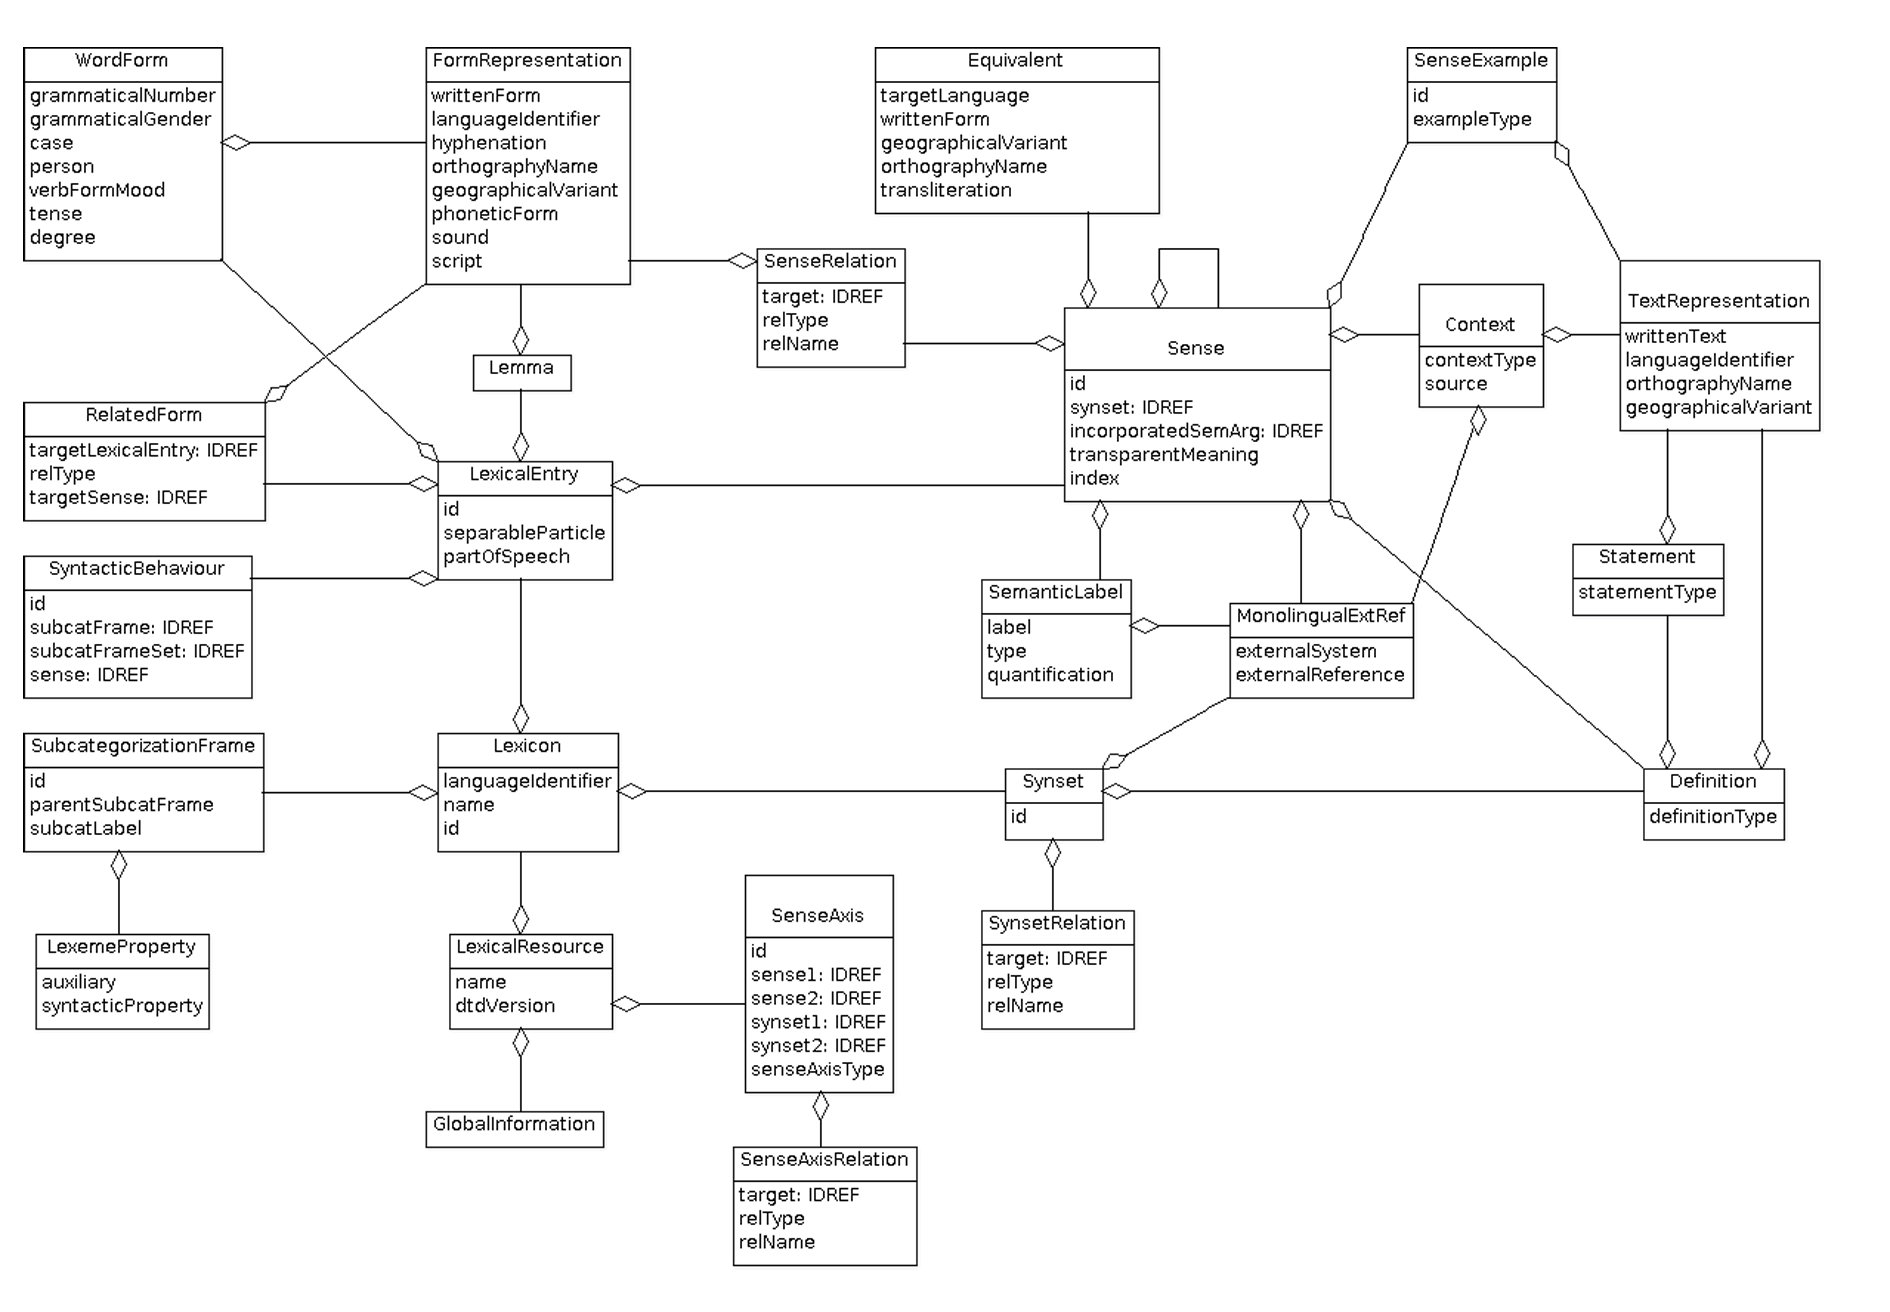
\includegraphics[width= 17cm, angle=90]{figures/lmfwktow}
  \caption{Overview of classes and data categories in our derived lexicon model}
  \label{fig:lmf}
\end{figure}

\begin{description} 
\item[Lexicon.]
In our \textsc{lmf} model, one unique \texttt{LexicalResource} instance which represents the complete resource consists of one or more \texttt{Lexicon} instances. In \textsc{uby-lmf}, each integrated resource is modeled as a separate \texttt{Lexicon}. Note further that \textsc{lmf} requires each \texttt{Lexicon} instance to belong to exactly one language (that is, having exactly one language identifier) -- a requirement that reflects the diversity of different languages at the morphosyntactic and lexical-syntactic level. Therefore, the multilingual resource OmegaWiki is split into separate \texttt{Lexicon} instances for each language while each language edition of Wiktionary constitutes one \texttt{Lexicon}.

\item[Lexical Entry and Sense.]
The lexical information is modeled using the \texttt{LexicalEntry} class, which is characterized by a \texttt{Lemma} (that is, a written form)  and a part-of-speech. Each entry in Wiktionary naturally  corresponds to exactly one \texttt{LexicalEntry}. In OmegaWiki, the \texttt{LexicalEntry} corresponds to  each lexicalization of a Defined Meaning. 
Each \texttt{LexicalEntry} may be connected to multiple instances of the \texttt{Sense} class modeling a certain meaning of the lexical entry. Word senses are explicitly encoded in Wiktionary and can therefore be straightforwardly used to populate the \texttt{Sense} instances. In OmegaWiki, word senses are represented by the Defined Meanings.

\item[Lexicographic Information.]
An integral part of our \textsc{lmf} model is the representation of the variety of lexicographic information found in Wiktionary and OmegaWiki, which is represented by different classes attached to \texttt{Sense}: While \texttt{Definition} and \texttt{SenseExample} are self-explanatory, the \texttt{Statement} class contains further knowledge about a \texttt{Sense}, such as etymological information. The \texttt{SemanticLabel} class contains labels for many different dimensions of semantic classification (for example, domain, register, style, sentiment) for word senses. Such labels are very useful, as they contain valuable hints on the situations or contexts in which a word sense is usually used. Relationships between word senses can be represented by means of paradigmatic relations, such as synonymy, antonymy, hyponymy that are modeled in the \texttt{SenseRelation} class. 

\item[Translation.]
In addition to the elements of \textsc{uby-lmf} described above, we introduce a new \texttt{Equivalent} class which is essential for any of the translation applications we have in mind. In this class, we store translation equivalents of a \texttt{Sense}, for example, the German translation \textit{Barsch} of \textit{bass}. Using the \texttt{Equivalent} class for this has been suggested before by \citet{Serasset12}, but -- as opposed to our model -- they represent translations at the word level rather than at the level of word senses.
\end{description}

For OmegaWiki, these translation equivalents are directly available via the lexicalizations in different languages attached to the same Defined Meaning. In Wiktionary, translation equivalents are encoded as links to other Wiktionary language editions. We create an instance of \texttt{Equivalent} for each of these translation links. The \texttt{Equivalent} class is designed to offer information that is vital for multilingual applications. Besides the written form of the translations and the target language, this includes: \texttt{transliteration} to encode different scripts (such as Cyrillic), \texttt{geographicalVariant} for representing a certain region in which the translated word is predominantly used (for example, Moscow), and \texttt{orthographyName} for storing a certain orthographic variant, such as the German orthography reform of 1996.

In the following sections, we will discuss the special issues of standardizing Wiktionary and OmegaWiki. More precisely, we will discuss classes, data categories, and general modeling questions concerning only one of the resources.

\subsection{Modeling Wiktionary in LMF}

As discussed in \sectref{sec:matuschek:wiktionary}, the guidelines for formatting entries in Wiktionary are not as strict as in OmegaWiki. 
This gap between the weakly structured Wiktionary articles and the rigidly structured \textsc{lmf} classes raises a number of challenges to our \textsc{lmf} representation of Wiktionary that we discuss below. Despite the heterogeneity of Wiktionary entries, we achieve a nearly lossless conversion of Wiktionary into the \textsc{uby-lmf} representation.

\begin{description}\sloppy
\item[Homonymy and Polysemy.]
Wiktionary distinguishes between homonymy and polysemy, as it is traditionally done in dictionaries. The former is used for words sharing the same form, but originating from different etymologies. Homonymy can be represented in our model by creating separate \texttt{LexicalEntry} instances for the homonymous entries in Wiktionary. The latter, polysemy, is used to encode different word senses sharing the same etymology. In this case, only one \texttt{LexicalEntry} is used. Consider the English noun \textit{post} as an example: There are separate entries in Wiktionary that refer to the Latin \textit{postis} (that is, the meaning of a \textit{doorpost}, \textit{pillar}) and the Latin \textit{positum} (that is, the meaning of a place where one is stationed). Hence, there are two instances of \texttt{LexicalEntry} representing the two different etymologies. Each of the lexical entries has multiple word senses modeling the polysemous meanings. For example, the distinction between a mail system (\textit{sent via post}) and the assigned station (\textit{leave one's post}).

\item[Underspecified Relations.]
An important type of information are paradigmatic relations such as synonymy, hyponymy, antonymy, etc.\ which are modeled using the \textsc{lmf} \texttt{SenseRelation} class. The \textsc{lmf} standard, however, originally considers each \texttt{Sense\-Relation} to be defined between two instances of \texttt{Sense} -- for example, between the message-system-related word senses of \textit{post} and \textit{mail}. In Wiktionary, only one of these word senses is explicitly defined: The first word sense of \textit{mail} encodes, for example, a synonymy link to \textit{post}, but does not give information about which word sense of \textit{post} is to be used. This conforms to the layout of most printed dictionaries, which list synonyms for a certain word sense without explicitly specifying the word sense of the synonym. The rationale behind this is that humans can easily disambiguate the different meanings of \textit{post} and do not require an explicit reference. To bridge the gap between this underspecification of Wiktionary's 
paradigmatic relations and our \textsc{lmf} representation, we introduce a new association relationship between the \texttt{SenseRelation} class and the \texttt{FormRepresentation} class. This way, we are able to store the word form of the relation targets without violating the model. In future work, we plan to automatically disambiguate the relations, so that we achieve a better structured representation of our resource.
\end{description}

In addition to those peculiarities of modeling Wiktionary in \textsc{lmf}, there is a number of information types found in Wiktionary, but not in OmegaWiki. We therefore use the following classes and data categories from the \textsc{uby-lmf} model.

\begin{description}\sloppy
\item[Phonetic Representation.]
Wiktionary contains a large number of phonetic representations explaining how a word is pronounced. For encoding this type of information, both \textsc{ipa} (International Phonetic Alphabet) and \textsc{sampa} (Speech Assessment Methods Phonetic Alphabet) notations are used; see \citet{Schlippe10} for more details on Wiktionary's representation of phonetic information. For our \textsc{lmf} representation, we use the \texttt{phoneticForm} data category of the \texttt{FormRepresentation} class to represent the pronunciation information. While pronunciations are not very useful for translations of written text, they are very helpful for foreign language learners. Often, there are sound files attached to Wiktionary that allow for listening to native speakers pronouncing a certain word. Such sound files can be linked from the model and hence be exploited for translation-related applications.

\item[Inflected Word Forms.]
A major problem when learning or translating to a foreign language is to use grammatically correct word forms. Although many inflected word forms are constructed using regular patterns, there are lots of exceptions that are difficult to remember or to manually encode into a translation system. The collaborative construction approach of Wiktionary can alleviate that, as a large number of people are involved and inflected word forms can quickly be encoded in a joint effort. In our model, we represent Wiktionary's inflected word forms using the \texttt{WordForm} class. For each word form, the grammatical number, gender, case, person, tense, etc.\ can be explicitly stored, such that an application using our resource can make use of this structured information.

\item[Related Words.]
In addition to paradigmatic relations between word senses, there are relations between word forms encoded in Wiktionary; for example, the nominalization \textit{driver} of the verb form \textit{(to) drive}. This type of relation is stored using the \texttt{RelatedForm} class. Of particular interest for translation-based applications are relations between similar word forms that are often mixed up by language learners or layman translators. There are, for example, relations between \textit{affect} and \textit{effect} or between the German words \textit{dediziert} (English:\ \textit{dedicated}) and \textit{dezidiert} (English: \textit{determined}).
\end{description}

\subsection{Modeling OmegaWiki in LMF}

While the fixed database structure of OmegaWiki as discussed in \sectref{sec:matuschek:omegawiki} ensures that the information can be consistently mapped to our \textsc{lmf} model,  there are still a number of issues which have to be addressed during the conversion process.

\begin{description}\sloppy
\item[Splitting Defined Meanings.]
As mentioned before, OmegaWiki does not have separate editions for each language. Instead, OmegaWiki is based on the notion of multilingual synsets, that is, language-independent concepts to which lexicalizations of the concepts are attached. As the \textsc{lmf} standard requires that a \texttt{Lexicon} is monolingual, we have to split OmegaWiki's Defined Meanings to create artificial language editions. For example, when populating our \textsc{lmf} model with a  \texttt{Lexicon} for the German OmegaWiki, we iterate over all Defined Meanings and only create those  \texttt{LexicalEntry}, \texttt{Sense}, etc.\ instances for which German lexicalizations are present. In turn, this means that concepts which are not lexicalized in German are simply left out of this \texttt{Lexicon}. The lexicalizations in the other languages are, however, not lost, but stored as translations using the \texttt{Equivalent} class. 

If more than one artificial language edition is created, there naturally exists a considerable overlap of concepts which are lexicalized in different languages. To express that the corresponding word senses in these languages refer to the same meaning, we utilize the \texttt{SenseAxis} class to link them. This is essentially the same mechanism as used to represent sense alignments between two resources (see \sectref{sec:matuschek:lmf:alignment} below). In other words, the information originally contained in OmegaWiki's Defined Meanings is preserved by modeling it as a cross-lingual sense alignment between the artificial language editions.


\item[Synsets and Synset Relations.]
As we explained earlier, the word senses of a \texttt{Lexical\-Entry} are derived from OmegaWiki's Defined Meanings. In our model, these senses are subsequently grouped into \texttt{Synsets}. This reflects the fact that the different lexicalizations of the same Defined Meaning describe the same concept and are thus synonyms. Consequently, as all relations in OmegaWiki are encoded between Defined Meanings, the paradigmatic relations expressed by \texttt{SenseRelation} instances can also be trivially transferred to \texttt{SynsetRelation} instances. That is to say, the structure of Omega\-Wi\-ki enforces that paradigmatic relations between synsets also hold for the contained senses and vice versa.

Another fact worth mentioning is that, other than Wiktionary, OmegaWiki also contains ontological (as opposed to linguistically motivated) relations -- for instance, the \textit{borders on} relation used to represent neighboring countries. This is very much in the spirit of OmegaWiki, being a collection of lexicalized concepts rather than a classic dictionary. This offers interesting ways of utilizing the multilingual information contained in our unified resource, such as using this ontological knowledge to enrich Wiktionary senses. Those relations are also modeled using the \texttt{SenseRelation} and \texttt{SynsetRelation} classes.


\item[Syntactic Properties.]
To a small extent, OmegaWiki allows encoding syntactic properties such as verb valency. While this only affects a small fraction of the entries for now, we assume that the importance of this will increase as the resource is edited and extended by the crowd. Thus, we integrate this information to make the transformation as complete as possible or even lossless, and also to prepare the ground for integrating OmegaWiki with resources which specifically focus on syntactic properties. To cater for this, we are utilizing the classes \texttt{SubcatFrame}, \texttt{LexemeProperty} and \texttt{SyntacticBehavior} which enable us to model all of the syntactic information available in OmegaWiki. Providing information on the proper grammatical usage of a word is important for finding a good translation, in particular if the target language uses different structures than the source language.
\end{description}


\subsection{Modeling sense alignments}
\label{sec:matuschek:lmf:alignment}

The word sense alignments between Wiktionary and OmegaWiki (as discussed in \sectref{sec:matuschek:alignment}) are modeled by means of \texttt{SenseAxis} instances. Note again that this is the same mechanism as for representing the multilingual information after splitting OmegaWiki into distinct language editions.

\subsection{Populating the LMF model}

As suggested by the \textsc{lmf} standard, we describe our model using a \emph{Document Type Definition} (\textsc{dtd}) that describes each class and their data categories. Based on this \textsc{dtd}, we developed a software for converting Wiktionary and OmegaWiki to our \textsc{lmf} representation. The software is designed for easy adaptation in case the resources change in the future, so that transformation to the common \textsc{lmf} model is still possible. This has the advantage that applications using the standardized resources can be continually kept up to date without the need to adapt to changes of a certain resource, as all adaptation effort is concentrated on the conversion software.

Our resource consists of four \texttt{Lexicon} instances: one for each of the German and English Wiktionary, and one for each of the German and English parts of OmegaWiki. It should be noted at this point that we use English and German as a case study on how this can be done -- the \textsc{lmf} converters allow to import other language editions with minor (Wiktionary) or no (OmegaWiki) modifications, and including more language editions into this resource is an important direction for future work. 

\tabref{tab:combinedstats} shows statistics about the most important \textsc{lmf} classes in our model regarding the single resources as well as the unified one. As can be seen, even with only two languages considered, we created a resource of an exceptional size with over 500,000 lexical entries and senses and well over 200,000 paradigmatic relations. Probably most important for translation applications, we also have almost 1,600,000 instances of the \texttt{Equivalent} class, which represent the translations (as discussed in \sectref{sec:matuschek:wiktionary} and \sectref{sec:matuschek:omegawiki}; a breakdown into single languages can be found in \tabref{tab:lang:trans}). In \tabref{tab:senseaxis}, we can see that  almost 90,000 \texttt{SenseAxis} instances have been created, over 25,000 of them stemming from our novel alignment of the two resources. Considering the around 58,000 senses in the English OmegaWiki, we have reached a fairly dense alignment of the two resources covering about half of OmegaWiki.

The final resource is published as an integral part of \textsc{uby} and available from our homepage \url{http://www.ukp.tu-darmstadt.de/uby/}. We offer a downloadable database, along with the \textsc{lmf} model, an easy-to-use \textsc{api}, the converters and accompanying documentation.

\begin{table}
  
  \begin{tabularx}{\textwidth}{X@{\qquad}rrrr}
\lsptoprule
    Resource & LexicalEntry & Sense & SenseRelation & Equivalent\\
    \midrule
    Wiktionary En & 335,749 & 421,848 &  22,313 & 694,282 \\
    OmegaWiki En  &  51,715 &  57,921 &   7,157 & 335,173 \\    
    Wiktionary De &  85,575 &  72,752 & 183,684 & 250,674 \\
    OmegaWiki De  &  30,967 &  34,691 &   7,165 & 304,590 \\  
\midrule
   Total &	504,006	  & 587,212 & 220,319 &  1,584,719 \\
\lsptoprule
  \end{tabularx}
  \caption{Statistics about the unified resource. The \texttt{Equivalent} class represents the translations found in each resource}
  \label{tab:combinedstats}
\end{table}


\begin{table}
  
  \begin{tabularx}{\textwidth}{lrQ}
    \lsptoprule
    Resource Pair &   SenseAxis & Comment/Information source\\
\midrule
OmegaWiki En -- OmegaWiki De &	58,785 & Orig. information by voluntary editors\\
OmegaWiki En -- Wiktionary En & 25,742  & Automatically produced alignment\\
\midrule
  Total &	84,527 	  & \\
  \lspbottomrule
  \end{tabularx}
  \caption{Sense alignment statistics}
  \label{tab:senseaxis}
\end{table}

\section{Conclusions and future work}
\label{sec:matuschek:conclusion}
In this article, we argued that collaboratively constructed multilingual lexical resources present a valuable source of knowledge for translation applications. They are maintained by a crowd of users, thus guaranteeing highly accurate and up to date information, while at the same time being available with almost no restrictions. We analyzed the two most prominent ones, Wiktionary and OmegaWiki in terms of (multilingual) content and structure and presented both their strengths and weaknesses: While the openness and flexibility of Wiktionary has attracted many users, leading to a resource of considerable size and richness, the non-standardized structure of entries also leads to difficulties in the integration into translation applications. OmegaWiki, on the other hand, does not suffer from this problem, but the self-imposed limitations to maintain integrity also constrain its expressiveness and, along with that, the range of information which can be represented 
in the resource. 

As a consequence of the content-related differences, we proposed a method for automatically aligning the two resources at the level of word senses with good precision. This yields a substantial increase of coverage, especially concerning available translations. In this respect, the aligned resource outperfoms either single resource by far, justifying the few alignment errors which are introduced in the process. To cater for the differences at the structural and representational level, we describe a nearly lossless and robust conversion of these two resources to a common, standardized representation based on the \textsc{uby-lmf} model \citep{EckleKohler12}, which we extended to also represent translation equivalents for word senses. As a result, we created a resource containing the English and German editions of OmegaWiki as well as Wiktionary, including translations into a multitude of additional languages, which is now an integral part of the unified resource \textsc{uby}. In summary, our resource has the following properties:

\begin{description}\sloppy
\item[Continuously updated lexical-semantic knowledge:] The frequently updated and extended knowledge in both resources can at any time be integrated into the unified resource as the conversion routines into the common model need no or only minor modifications in the future. This also relieves the end user from the burden of adapting their application to changes in the underlying resources as the unified output model remains stable. 
\item[High coverage:] The alignments at word sense level significantly improve  upon the available information in the isolated resources, which is very valuable for translation purposes and other applications. The proposed generic alignment framework makes sure that alignments for future revisions of both resources can be performed with little effort.

  
\item[A standardized structure:] The \textsc{lmf}-based model, supported by a corresponding database or \textsc{xml} schema, ensures that the resource can be queried with consistent and reliable results. 
\item[Elaborate structure:] The structure of the \textsc{lmf} model is elaborate and expressive enough to cater for a wide range of lexicographic information in different languages, so that an almost complete representation of the underlying resources is possible.
\item[Interoperability:] The resource is not only in a format which is machine readable, but it is also compliant to existing \textsc{kyoto} standards to allow for easy reuse and integration into applications.
\end{description}

There are many directions to pursue for future work. First of all, we want to apply and extend our resource alignment approach to other pairs of lexicographic resources. A special focus will be on creating additional alignments between expert-built\footnote{Note that ``expert'' in this context refers to linguists (language experts) and not professional translators.} and collaboratively constructed resources to actively exploit the complementary information in different types of resources, which have been constructed following different paradigms. The recently published alignment between Wiktionary and FrameNet based on the same approach \citep{TUD-CS-2013-0082} is a first step in this direction.

Another goal is to apply the graph-based method for sense alignment we recently introduced \citep{TUD-CS-2013-0057} to Wiktionary and OmegaWiki to validate its applicability in a setup with two collaboratively constructed resources. In this context, we will also explore how the combined evidence from already existing alignments could be used to infer new ones; here, graph-based methods operating on the graph of aligned senses seem to be a viable option. Also, the inclusion of more language editions of Wiktionary and OmegaWiki and, more generally, an improved treatment of cross-lingual alignments  should be tackled in the future work.

A crucial point for further research is the actual usage of our unified resource in translation applications. The integration into a computer-aided translation environment or an \textsc{smt} system as mentioned in the introductory section is particularly interesting. For this, we would be interested in collaborating with researchers from the (machine) translation community in order to assess the usefulness of aligned resources, and also to discover aspects in which further improvement is necessary, for example, regarding coverage or precision.

Lastly, further development of the \textsc{api}\footnote{\url{https://code.google.com/p/uby/}} and the accompanying Web interface\footnote{\url{https://uby.ukp.informatik.tu-darmstadt.de/webui}} is necessary to make the resource more easily accessible to as many researchers and end users as possible. We especially deem the interface important as visually assessing and evaluating the generated sense alignments becomes increasingly difficult for larger lexical resources.

\section*{Acknowledgements}
This work has been supported by the Volkswagen Foundation as part of the Lichtenberg Professorship Program under grant No. I/82806 and by the Hessian research excellence program ``Landes-Offensive zur Entwicklung Wissenschaftlich-\"{o}konomischer Exzellenz (\textsc{loewe})'' as part of the research center ``Digital Humanities''. We would like to thank Judith Eckle-Kohler, Silvana Hartmann, Tri-Duc Nghiem, Elisabeth Niemann, Yevgen Chebotar and Zijad Maksuti for their contributions to this work. We also thank the anonymous reviewers for their helpful remarks.


\sloppy
\printbibliography[heading=subbibliography,notkeyword=this]

\end{document}
